\documentclass[pdf]{beamer}
%\documentclass[notes]{beamer}
%\documentclass{beamer}
\usepackage[utf8]{inputenc}
\usepackage{lmodern}
\usepackage{colortbl}
\usepackage{adjustbox}
%\usepackage{scrextend}
%\changefontsizes{7.5pt}


\makeatletter
\makeatother
\usepackage{graphicx}

\mode<presentation>{\usetheme{Warsaw}}
%\mode<presentation>{\usetheme{Madrid}}
%% preamble
\title{Métodos multivariados de Análisis de Datos}
\subtitle{Filtro de spam personalizado}

\author{
Ricardo Cruz Sánchez \\
  \and
Rolando Corona Jiménez
}

\institute[CIMAT]{CIMAT}

\AtBeginSection[]{%
\begin{frame}
    \tableofcontents[currentsection, subsectionstyle=show/show/hide]
\end{frame}
}

\begin{document}

\begin{frame}
\titlepage
\end{frame}

%\AtBeginSubsection[]
%{
%  \begin{frame}<beamer>
%    \frametitle{Contenido}
%    \tableofcontents[currentsection,currentsubsection]
%  \end{frame}
%}



\section{Introducción}
\begin{frame}{Spam}

\end{frame}


\begin{frame}{Repositorio}
\begin{itemize}

\item https://github.com/rolandocj/proyecto-pizzas/tree/develop
\end{itemize}

\end{frame}



\section{Análisis exploratorio.}

\subsection{Descripción del conjunto de datos.}

\begin{frame}{Conjunto de datos}
El conjunto de datos proviene de una serie de correos electrónicos del personal de la empresa HP. Los correos etiquetados como spam fueron proporcionados por el administrador del servidor de correo de la empresa, mientras que los correos que no están etiquetados como spam corresponden a correos personales y de trabajo de George Forman, es por ello que palabras como \textit{george} o código de área $650$ son indicadores de no spam. La base de datos fue creada por Mark Hopkins, Erik Reeber, George Forman y Jaap Suermondt de Hewlett-Packard Labs.
\end{frame}

\begin{frame}
\begin{table}[ht]
\centering
\begin{tabular}{|l|l|l|}
\hline
Spam     & $1813$ & $39.4 \%$ \\ \hline
Non-Spam & $2788$ & $60.6 \%$ \\ \hline
\end{tabular}
\caption{Distribución de clases.}
\label{t_dist}
\end{table}
\end{frame}

\subsection{Diccionario de datos}

\begin{frame}
En total se cuentan 4601 observaciones, de las cuales 1813 fueron etiquetadas como spam, que corresponde al $39.4\%$ del total. Las observaciones están representadas a través de un conjunto de 58 atributos: $57$ variables cuantitativas y una variable cualitativa nominal de clase. Ninguno de los atributos presenta datos faltantes. 
\end{frame}

\begin{frame}
Los 58 atributos se pueden agrupar en:
\begin{itemize}
	\item 48 variables cuantitativas continuas con rango $[0,100]$, de la forma word\_freq\_WORD, que indica el porcentaje de palabras en el correo que coinciden con WORD, es decir:
	$$word\_freq\_WORD = 100 \times \dfrac{\#\text{apariciones de WORD en el correo}}{\#\text{total de palabras en el correo}}$$
	
	\item 6 variables cuantitativas continuas con rango $[0,100]$, de la forma char\_freq\_CHAR, que indica el porcentaje de caracteres en el correo que coinciden con CHAR, es decir:	
		$$char\_freq\_CHAR = 100 \times \dfrac{\#\text{apariciones de CHAR en el correo}}{\#\text{total de caracteres en el correo}}$$
\end{itemize}
\end{frame}

\begin{frame}
\begin{itemize}
	\item 1 variable cuantitativa continua \textsf{capital\_run\_length\_average} con rango $[0,\infty)$, que es igual a longitud media de las secuencias contiguas de letras mayúsculas que aparecen en el correo.
	
	\item 1 variable cuantitativa discreta \textsf{capital\_run\_length\_longest} con rango $[0,\infty)$, que es igual a la longitud de la secuencia contigua de letras mayúsculas más larga que aparece en el correo.
	
	\item 1 variable cuantitativa discreta \textsf{capital\_run\_length\_total} con rango $[0,\infty)$, que es igual a la suma de las longitudes de las secuencias contiguas de letras mayúsculas que aparecen en el correo.
	
	\item 1 variable nominal de clase con valores en $\{0, 1\}$, que indica si el correo se considera spam (1) o no (0).
\end{itemize}

La documentación del conjunto de datos no indica los criterios para la selección de las 48 palabras y 6 caracteres usados para la definición de sus correspondientes variables.

\end{frame}
 
\begin{frame}
\begin{table}[ht]
\centering
\begin{tabular}{|l|l|l|l|l|l|}
\hline
make     & order     & business & hp     & data       & cs         \\ \hline
address  & mail      & email    & hpl    & 415        & meeting    \\ \hline
all      & receive   & you      & george & 85         & original   \\ \hline
3d       & will      & credit   & 650    & technology & project    \\ \hline
our      & people    & your     & lab    & 1999       & re         \\ \hline
over     & report    & font     & labs   & parts      & edu        \\ \hline
remove   & addresses & 000      & telnet & pm         & table      \\ \hline
internet & free      & money    & 857    & direct     & conference \\ \hline
\end{tabular}
\caption{Palabras que corresponden a las variables de tipo word\_freq\_WORD.}
\label{t_words}
\end{table}
\end{frame}

\begin{frame}
\begin{table}[ht]
\centering
\begin{tabular}{|l|}
\hline
;   \\ \hline
(   \\ \hline
{[} \\ \hline
!   \\ \hline
\$  \\ \hline
\#  \\ \hline
\end{tabular}
\caption{Caracteres que corresponden a las variables de tipo char\_freq\_CHAR.}
\label{t_chars}
\end{table}
\end{frame}

\section{Métricas para clasificación binaria.}


\begin{frame}
\begin{figure}[h]
\centering
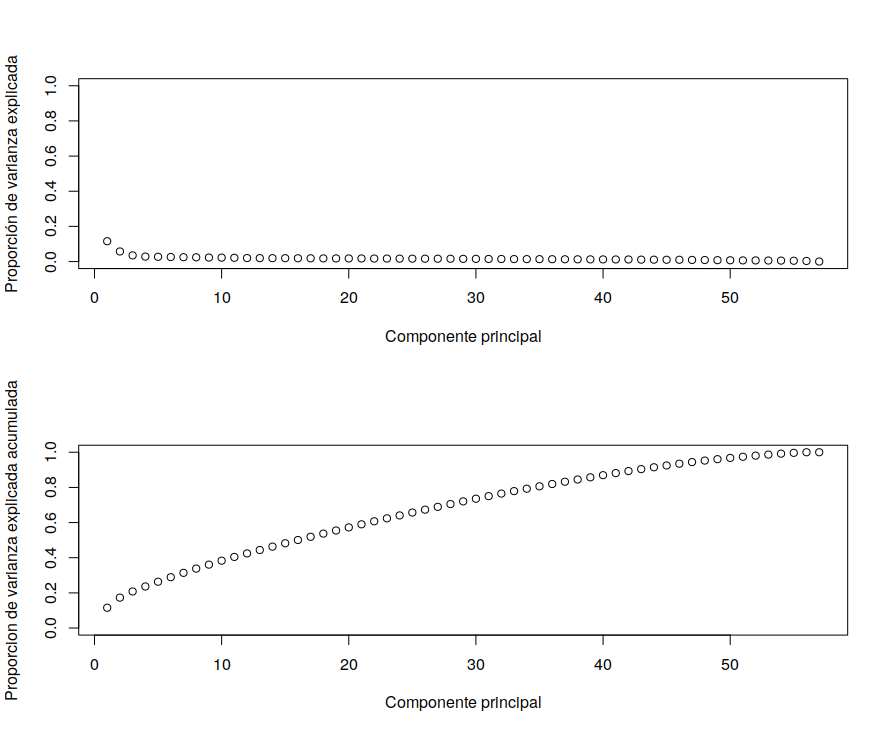
\includegraphics[scale=.65]{images/pca.png} 
\label{i1}
\caption{Conteo de registros por marca}
\end{figure}
\end{frame}

\begin{thebibliography}{1}

\bibitem{cr98}
Lorrie Faith Cranor and Brian A. LaMacchia. 1998. Spam!. Commun. ACM 41, 8 (August 1998), 74-83. 

\bibitem{fe19}
Emilio Ferrara. 2019. The history of digital spam. Commun. ACM 62, 8 (July 2019), 82-91. 

\bibitem{ha01}
Hastie, T., Tibshirani, R.,, Friedman, J. (2001). The Elements of Statistical Learning. New York, NY, USA: Springer New York Inc.. 

\bibitem{so09}
Marina Sokolova and Guy Lapalme. 2009. A systematic analysis of performance measures for classification tasks. Inf. Process. Manage. 45, 4 (July 2009), 427-437. 

\end{thebibliography}



\end{document}
